\documentclass[border=6pt]{standalone}
\usepackage{lmodern}
\usepackage[T1]{fontenc}
\usepackage{amsmath,amssymb}
\usepackage{bm}
\usepackage{xcolor}
\usepackage{tikz}
\usetikzlibrary{arrows.meta,positioning}
\definecolor{cblue}{HTML}{2F7DC8}
\definecolor{cgreen}{HTML}{4E8E2A}
\definecolor{cink}{HTML}{2B2B2B}
\newcommand{\Exp}{\mathbb{E}}
\tikzset{>={Stealth[length=2.2mm]},
  band/.style={rounded corners=4pt,draw=cblue!70,line width=0.7pt},
  clab/.style={font=\footnotesize,text=cink,align=left},
}
\begin{document}
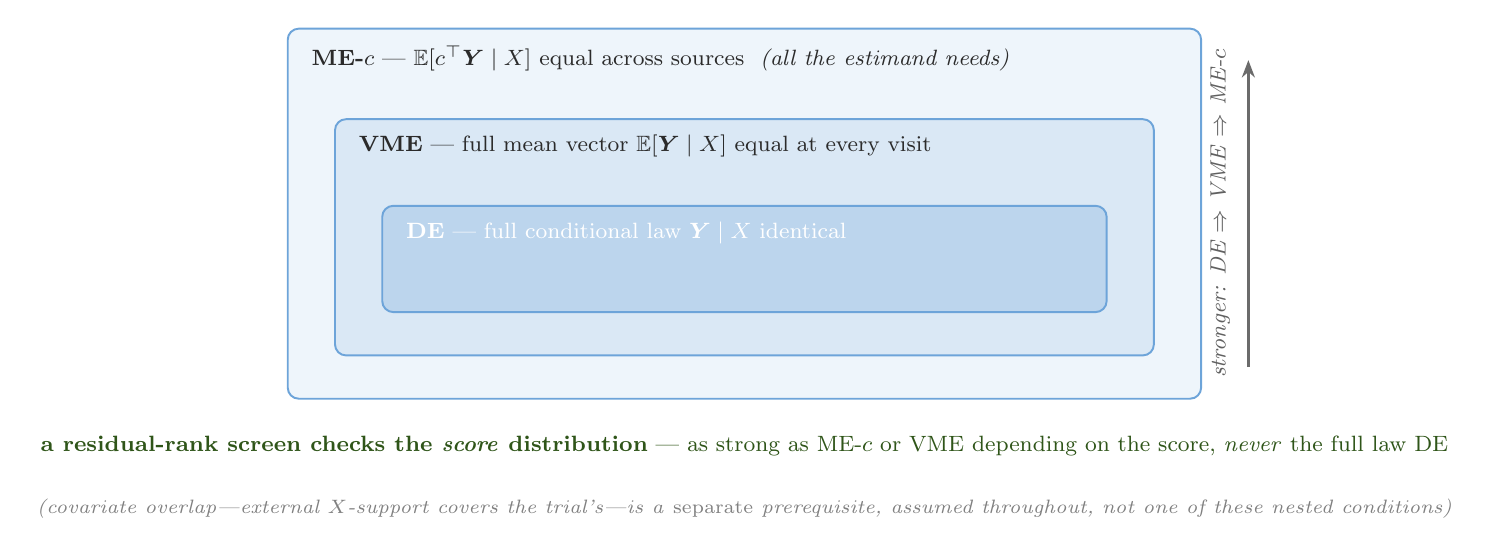
\begin{tikzpicture}[font=\small]
  % three nested outcome-compatibility conditions: DE => VME => ME-c
  \draw[band,fill=cblue!8]  (0,0)      rectangle (11.6,4.7);
  \draw[band,fill=cblue!18] (0.6,0.55) rectangle (11.0,3.55);
  \draw[band,fill=cblue!32] (1.2,1.1)  rectangle (10.4,2.45);

  \node[clab,anchor=north west] at (0.18,4.6)  {\textbf{ME-$c$} --- $\Exp[c^{\top}\bm Y\mid X]$ equal across sources \ \textit{(all the estimand needs)}};
  \node[clab,anchor=north west] at (0.78,3.47) {\textbf{VME} --- full mean vector $\Exp[\bm Y\mid X]$ equal at every visit};
  \node[clab,anchor=north west,text=white] at (1.38,2.37) {\textbf{DE} --- full conditional law $\bm Y\mid X$ identical};

  \draw[->,cink!70,line width=1.0pt] (12.2,0.4) -- (12.2,4.3)
        node[midway,rotate=90,anchor=south,font=\footnotesize\itshape,text=cink!75,yshift=1mm]{stronger: DE $\Rightarrow$ VME $\Rightarrow$ ME-$c$};

  \node[clab,text=cgreen!60!black,align=center,anchor=north] at (5.8,-0.35)
     {\textbf{a residual-rank screen checks the \emph{score} distribution} --- as strong as ME-$c$ or VME depending on the score, \emph{never} the full law DE};
  \node[clab,text=cink!60,align=center,anchor=north,font=\scriptsize\itshape] at (5.8,-1.15)
     {(covariate overlap---external $X$-support covers the trial's---is a \emph{separate} prerequisite, assumed throughout, not one of these nested conditions)};
\end{tikzpicture}
\end{document}
